\documentclass[]{article}

\PassOptionsToPackage{numbers,compress}{natbib}

\usepackage[]{neurips_2021}
\usepackage[utf8]{inputenc} 
\usepackage[T1]{fontenc}    
\usepackage{hyperref}       
\usepackage{url}            
\usepackage{booktabs}       
\usepackage{nicefrac}       
\usepackage{microtype}      
\usepackage{amsfonts,amsmath,amssymb}	
\usepackage{mathtools}
\usepackage{lipsum}
\usepackage{xspace}
\usepackage[dvipsnames]{xcolor}

\newcommand{\Fermi}{\emph{Fermi}\xspace}
\newcommand{\HEALPix}{\texttt{HEALPix}\xspace}
\newcommand{\dd}{\mathrm{d}}
\newcommand{\vect}[1]{\boldsymbol{\mathbf{#1}}}

\definecolor{linkcolor}{rgb}{0.7752941176470588, 0.22078431372549023, 0.2262745098039215}
\hypersetup{colorlinks=true,
linkcolor=linkcolor,
citecolor=linkcolor,
urlcolor=linkcolor,
linktocpage=true,
pdfproducer=medialab,
}

\title{Characterizing $\gamma$-rays maps of the Galactic Center \\ with neural density estimation}

\author{
Siddharth Mishra-Sharma \\
Massachusetts Institute of Technology \\
The NSF AI Institute for Artificial Intelligence and Fundamental Interactions \\
Harvard University \\ 
New York University \\
\texttt{sm8383@nyu.edu} \\
}

\begin{document}

\maketitle

\begin{abstract}
Machine learning methods have enabled new ways of performing inference on high-dimensional datasets modeled using complex simulations. We leverage recent advancements in simulation-based inference in order to characterize the contribution of various modeled components to $\gamma$-ray data of the Galactic Center recorded by the \Fermi satellite. A specific goal here is to differentiate ``smooth'' emission, as expected for a dark matter origin, from more ``clumpy'' emission expected for a population of relatively bright, unresolved astrophysical point sources. Compared to traditional techniques based on the statistical distribution of photon counts, our machine learning-based method based on density estimation using normalizing flows is able to utilize more of the information contained in a given model of the Galactic Center emission, and in particular can perform posterior parameter estimation while accounting for pixel-to-pixel spatial correlations in the $\gamma$-ray map. 
% On application to real \Fermi data, the method generically attributes a smaller fraction of the flux associated with the excess to an unresolved point source population compared to traditional approaches.

% The nature of the \Fermi $\gamma$-ray Galactic Center Excess (GCE) has remained a persistent mystery for over a decade. Although the excess is broadly compatible with emission expected due to dark matter annihilation, an explanation in terms of a population of unresolved astrophysical point sources \emph{e.g.}, millisecond pulsars, remains viable. The effort to uncover the origin of the GCE is hampered in particular by an incomplete understanding of diffuse emission of Galactic origin. This can lead to spurious features that make it difficult to robustly differentiate smooth emission, as expected for a dark matter origin, from more ``clumpy'' emission expected for a population of relatively bright, unresolved point sources. 
\end{abstract}

\section{Introduction}
\label{sec:intro}

Dark matter (DM) represents one of the major unsolved problems in particle physics and cosmology today. The traditional Weakly-Interacting Massive Particle (WIMP) paradigm envisions production of dark matter in the early Universe through freeze-out of dark sector particles weakly coupled to the Standard Model (SM) sector. In this scenario, one of the most promising avenues of detecting a dark matter signal is through an observation of excess $\gamma$-ray photons at $\sim\mathrm{GeV}$ energies from DM-rich regions of the sky.  The \Fermi $\gamma$-ray Galactic Center Excess (GCE), first identified over a decade ago using data from the \Fermi Large Area Telescope (LAT)~\cite{Atwood:2009ez}, is an excess of photons in the Galactic Center with properties---such as energy spectrum and spatial morphology---broadly compatible with expectation due to annihilating DM.% produced through the cascade of SM particles resulting from DM self-annihilation. 

The high dimensionality of $\gamma$-ray data has traditionally necessitated a description of the photon map in terms of hand-crafted summary quantities \emph{e.g.}, the probability distribution of photon counts~\cite{Lee:2014mza,Lee:2015fea} or a wavelet decomposition of the photon map~\cite{Bartels:2015aea,Balaji:2018rwz,McDermott:2015ydv,Zhong:2019ycb}, in order to enable computationally tractable analyses. While effective, this reduced description necessarily involves loss of information compared to that contained in the original $\gamma$-ray map. On the other hand, recent developments in machine learning have enabled analysis techniques that can extract more information from high-dimensional datasets, using more of the information contained in the models of $\gamma$-ray emission. Machine learning methods have recently shown promise for analyzing $\gamma$-ray data~\cite{Caron:2021map} and specifically for understanding the nature of the \Fermi GCE~\cite{List:2020mzd,List:2021aer,Caron:2017udl}.

Here, we showcase a complementary approach that leverages recent developments in simulation-based inference (SBI, also referred to as likelihood-free inference; see, \emph{e.g.}, Ref.~\cite{cranmer2020frontier} for a recent review)
%  ~\cite{Alsing:2019xrx,Brehmer:2018eca,Brehmer:2018hga,Brehmer:2018kdj,Brehmer:2020cvb,Cranmer:2015bka,cranmerFrontierSimulationbasedInference2020,durkanContrastiveLearningLikelihoodfree2020,greenbergAutomaticPosteriorTransformation2019,Hermans:2019ioj,lueckmannBenchmarkingSimulationBasedInference2021,lueckmannLikelihoodfreeInferenceEmulator2019,pacchiardiGeneralizedBayesianLikelihoodFree2021,papamakariosFastEpsilonFree2018,papamakariosSequentialNeuralLikelihood2019,wiqvistSequentialNeuralPosterior2021,zhaoValidatingConditionalDensity2021} 
in order to weigh in on the nature of the GCE. In particular, we use conditional density estimation techniques based on normalizing flows~\cite{papamakarios2019normalizing,rezende2015variational} to characterize the contributions of various modeled components, including ``clumpy'' PS-like and ``smooth'' DM-like emission spatially tracing the GCE, to the $\gamma$-ray photon sky at $\sim\mathrm{GeV}$ energies in the Galactic Center region. Rather than using hand-crafted summary statistics, we employ a graph-based convolutional neural network architecture (previously utilized in Refs.~\cite{List:2020mzd,List:2021aer}) in order to extract summary statistics from $\gamma$-ray maps optimized for the downstream task of estimating the distribution of parameters characterizing the contribution of modeled components to the GCE. Unlike traditional approaches based on the statistics of photon counts, this approach lets us capture more of the information contained in a model of the Galactic Center emission, and in particular implicitly uses the distribution of correlations between pixels as an additional discriminating handle. This fact makes our method more resilient to certain systematic uncertainties associated with model mis-specification as compared to traditional approaches.

\section{Model and inference}
\label{sec:model}

\paragraph{The forward model} We use the datasets and spatial templates from Refs.~\cite{rodd_nicholas_safdi_siddharth_2016,Mishra-Sharma:2016gis} to create simulated maps of \Fermi data in the Galactic Center region. 
% The data and templates used correspond to 413 weeks of \Fermi-LAT Pass 8 data collected between August 4, 2008 and July 7, 2016. The top quarter of photons by quality of PSF reconstruction in the energy range 2--20~GeV and event class \texttt{ULTRACLEANVETO} are used. The recommended quality cuts are applied, corresponding to zenith angle less than 90$^\circ$, \texttt{LAT\_CONFIG} = 1, and \texttt{DATA\_QUAL} $> 0.1$.\footnote{\url{https://fermi.gsfc.nasa.gov/ssc/data/analysis/documentation/Cicerone/Cicerone_Data_Exploration/Data_preparation.html}} 
The maps are spatially binned using the \texttt{HEALPix}~\cite{Gorski:2004by} pixelization scheme with resolution parameter \texttt{nside}=128, roughly corresponding to pixel area $\sim 0.5\,\mathrm{deg}^2$. The inner region of the Galactic plane, where the observed emission is especially difficult to model, is masked at latitudes $|b| < 2^\circ$, and a radial cut $r < 25^\circ$ defines our region of interest (ROI) in the Galactic Center.

The simulated data maps are a combination of diffuse (alternatively referred to as smooth or Poissonian) and PS contributions. The smooth contributions include \emph{(i)}~the Galactic diffuse foreground emission~\cite{Buschmann:2020adf}, \emph{(ii)}~spatially isotropic emission accounting for, \emph{e.g.}, uniform emission from unresolved sources of extragalactic origin, \emph{(iii)}~emission from resolved PSs included in the \Fermi 3FGL catalog~\cite{Fermi-LAT:2015bhf}, and \emph{(iv)}~lobe-like emission associated with the \Fermi bubbles~\cite{Su:2010qj}. Finally, \emph{(v)}~Smooth DM-like emission is modeled using a line-of-sight integral of the (squared) generalized Navarro-Frenk-White (NFW)~\cite{Navarro:1995iw,Navarro:1996gj} profile, $\rho_\mathrm{gNFW}(r) \propto {\left(r / r_{\mathrm s}\right)^{-\gamma}\left(1+r / r_{\mathrm s}\right)^{-3+\gamma}}$ with inner slope $\gamma=1.2$ motivated by previous GCE analyses~\cite{Gordon:2013vta,Daylan:2014rsa,Zhou:2014lva}. The total smooth component is obtained as a Poisson realization of a linear combination of these spatial templates. % Here, $r$ is the radial distance from the Galactic Center, $r_{\mathrm s}=20\,\mathrm{kpc}$ is the Milky Way scale radius, and we take $R_\odot = 8.2\,\mathrm{kpc}$ as the distance to the Galactic Center~\cite{2020arXiv201202169B,2019A&A...625L..10G}.

Assuming the locations of individual PSs are not known a-priori, the statistics of multiple PS populations can be completely specified through \emph{(i)} their spatial distribution, described by templates $T^p$ discretized over pixels $p$, \emph{(ii)} the distribution of expected photon counts $S$ contributed by each PS, $p(S)$, and \emph{(iii)} the distribution of the number of PSs for each population.  Additionally, the modeled instrumental point-spread function quantifies the spatial distribution of photon counts sourced by individual PS around its location due to the finite angular resolution of the instrument.
Here, we parameterize the distributions of photon counts $S$ contributed by each PS through a doubly-broken power law
% \begin{equation}
% \label{eq:scd_bpl}
% p(S\mid\theta_\mathrm{PS})\propto \left\{\begin{array}{lc}
% \left(\frac{S}{S_{\mathrm b, 1}}\right)^{-n_{1}}, & S \geq S_{\mathrm b, 1} \\
% \left(\frac{S}{S_{\mathrm b, 1}}\right)^{-n_{2}}, & S_{\mathrm b, 1}>S \geq S_{\mathrm b, 2} \\
% \left(\frac{S_{\mathrm b, 2}}{S_{\mathrm b, 1}}\right)^{-n_{2}}\left(\frac{S}{S_{\mathrm b, 2}}\right)^{-n_{3}}, & S_{\mathrm b, 2}>S
% \end{array}\right.
% \end{equation}
specified by the break locations $\{S_{\mathrm b, 1}, S_{\mathrm b, 2}\}$, spectral indices (slopes) $\{n_1, n_2, n_3\}$, and appropriately normalized to unity. Together, we denote these parameters by $\theta_\mathrm{PS}$.

The PS components of the simulated \Fermi map are created as follows, practically implemented using the code package \texttt{NPTFit-Sim}~\cite{NPTFit-Sim}. The total number of PSs to be simulated is drawn as $n \sim \mathrm{Pois}(n\mid n_\mathrm{pix}\lambda)$, where $n_\mathrm{pix}$ is the number of pixels in the ROI. The sample of PS angular positions is drawn from a PDF constructed by linearly interpolating the relevant pixel-wise spatial template $T^p$; $\{r_n\} \sim p(r) \propto T(r)$. The expected number of photons emitted by each PS, indexed by $i$, is drawn by sampling from the mean source-count distribution, $S \sim p\left({S}\mid\theta_\mathrm{PS}\right)$, and scaling to correct for non-uniform exposure of the satellite. The actual sample of photon counts emitted by the simulated PSs, $\{x_n\}$, is taken to be a Poisson realization of this expectation. 
% Given the angular positions of and photon counts emitted by PSs $\{r_n, x_n\}$, the radial coordinates of photons relative to the positions of PSs are drawn following the modeled \Fermi PSF. 
The procedure is repeated for each PS population, and the final simulated PS map is constructed by binning the sampled photon positions within the ROI according to the pixelization scheme used. The total map is obtained by combining the simulated diffuse and PS components. The inclusion of PSs in the forward model introduced a large number of latent variable---the positions and fluxes associated with each PS---and renders the full likelihood of the model intractable.

Modeled PS populations are often compactly described through the so-called source-count distribution (SCD) $\dd^2 N /\dd S \dd\Omega$, which quantifies the differential number density of sources per unit angular area emitting $S$ photons in expectation. The source-count distribution jointly describes the distribution of photon counts from individual PSs $p(S\mid\theta_\mathrm{PS})$ and their mean per-pixel abundance $\lambda$, and is related to these as ${\dd^2 N}{\dd S\dd\Omega}=\lambda \, p(S\mid\theta_\mathrm{PS}) / \Omega_\mathrm{pix}$
% We note that these parameters specify the {spatially-averaged} properties of the PS population---variation due to non-uniform exposure of the LAT instrument is accounted for in putting down simulated photon counts. 
where the the pixel area $\Omega_\mathrm{pix}$ is used to convert the per-pixel source count to per-area, agnostic to pixel size. We will present our results in terms of the source fluxes ($\dd^2 N /\dd F\dd\Omega$), with the conversion $S = \langle \epsilon \rangle F$ where $\langle \epsilon \rangle$ is the mean exposure in the region considered. Two PS populations are modeled---\emph{(i)} those correlated with the GCE, following an NFW profile, and \emph{ii} those tracing the Galactic disk, spatially modeled using a doubly exponential profile with scale height $z_\mathrm{s} = 0.3\,\mathrm{kpc}$ and radius $R_\mathrm{d} = 5\,\mathrm{kpc}$

The forward model is thus specified by a total of 18 parameters---6 for the overall normalizations of the Poissonian templates, and $6\times2$ parameters modeling the source-count distributions associated with GCE-correlated and disk-correlated PS populations $\{\langle S^{\rm PS} \rangle, n_1, n_2, n_3, S_{\mathrm b, 1}, S_{\mathrm b, 2}\}$. $\langle S^{\rm PS} \rangle$ denotes the mean per-pixel counts contributed by a given PS population, and parameterizes their overall abundance.

\paragraph{Inference with likelihoods based on simplified data representations} The 1-point PDF (probability distribution function) framework, first introduced in the context of $\gamma$-ray analyses in Ref.~\cite{Malyshev:2011zi} and extended in Refs.~\cite{Lee:2014mza,Lee:2015fea} under the name of non-Poissonian template fitting (NPTF), considers a simplification of the problem by computing the pixel-wise likelihood assuming each pixel to be statistically independent (\emph{1-point} then referring to values over individual, independent spatial positions in the sky). This significantly reduces the latent space dimensionality by eliminating the positions of individual PSs as latent variables, localizing them within a pixel and modulating their expected abundance by the modeled spatial template (\emph{e.g.}, GCE-correlated or disk-correlated in our case). Here, we use this method as a comparison point, and sample the posterior associated with parameters of interest with \texttt{dynesty}~\cite{Speagle_2020} using the likelihood from \texttt{NPTFit}~\cite{Mishra-Sharma:2016gis}.

\paragraph{Extracting representative features from $\gamma$-ray maps} Rather than relying on hand-crafted data summaries, a neural network is used to extract representative features $s_\varphi(x)$ of the data $x$ optimized for the downstream density estimation task. We use the \texttt{DeepSphere} architecture~\cite{defferrard2020deepsphere,Perraudin:2018rbt,deepsphere_rlgm} with a configuration similar to and inspired by that employed in Ref.~\cite{List:2020mzd}. \texttt{DeepSphere} is a graph-based spherical convolutional neural network architecture tailored to data sampled on a sphere, and in particular is able to leverage the hierarchical structure of data in the \texttt{HEALPix} representation. This makes it well-suited for our purposes. The architecture consists of graph convolutional layers which, following a ReLU nonlinearity, coarsens the pixel representation by a factor of 4 with max pooling while doubling the number of feature dimensions until a maximum of 256. The output of the final convolution layer is passed through a fully connected neural network with 1024 hidden units before outputting 128 summaries.

\paragraph{Simulation-based inference with normalizing flows} Simulation-based inference (SBI) refers to a class of methods for performing inference when the data-generating process does not have a tractable likelihood. This is the case for the forward model used here, where the presence of a large number of PSs leads to a large latent space. We approximate the joint posterior over the parameters of interest $\theta$ given a $\gamma$-ray map $x$ through a distribution $\hat p_\phi(\theta\mid s_\varphi(x))$ conditioned on summaries $s_\varphi(x)$ from simulated samples $\{x\}$. The conditioned posterior distribution is parameterized by $\phi$ and defined via normalizing flows~\cite{papamakarios2019normalizing,rezende2015variational}, which are a class of models that provide an efficient way of modeling high-dimensional probability distributions. Specifically, we use Masked Autoregressive Flows (MAFs)~\cite{10.5555/3294771.3294994} to define the flow transformation. We use 8 MAF transformations, each made up of a 2-layer masked autoregressive neural network~\cite{germain2015made} with 128 hidden units and $\tanh$ activations. 
% The ordering of parameters in the autoregressive sequence is randomly permuted between successive transformations in order to reduce dependence on the specific ordering of input variables. 
Each transformation is conditioned on summaries $s_\varphi(x)$ by including these as additional inputs into the transformation blocks.

Normalizing flows allow for tractable density evaluation, and $\log \hat p_\phi(\theta\mid s_\varphi(x))$ is used as the training objective to simultaneously optimize parameters $\{\phi,\varphi\}$ associated with the convolution and flow neural networks, respectively. $10^6$ samples from the forward model are produced, with 15\% of these held out for validation. The model is trained for up to 30 epochs with early stopping, using a batch size of 256. The \texttt{AdamW} optimizer~\cite{kingma2017adam,loshchilov2019decoupled} is used with initial learning rate $10^{-3}$ and weight decay $10^{-5}$, with learning rate decayed through cosine annealing.

\section{Application to \Fermi data}
\label{sec:experiments}

%
\begin{figure}
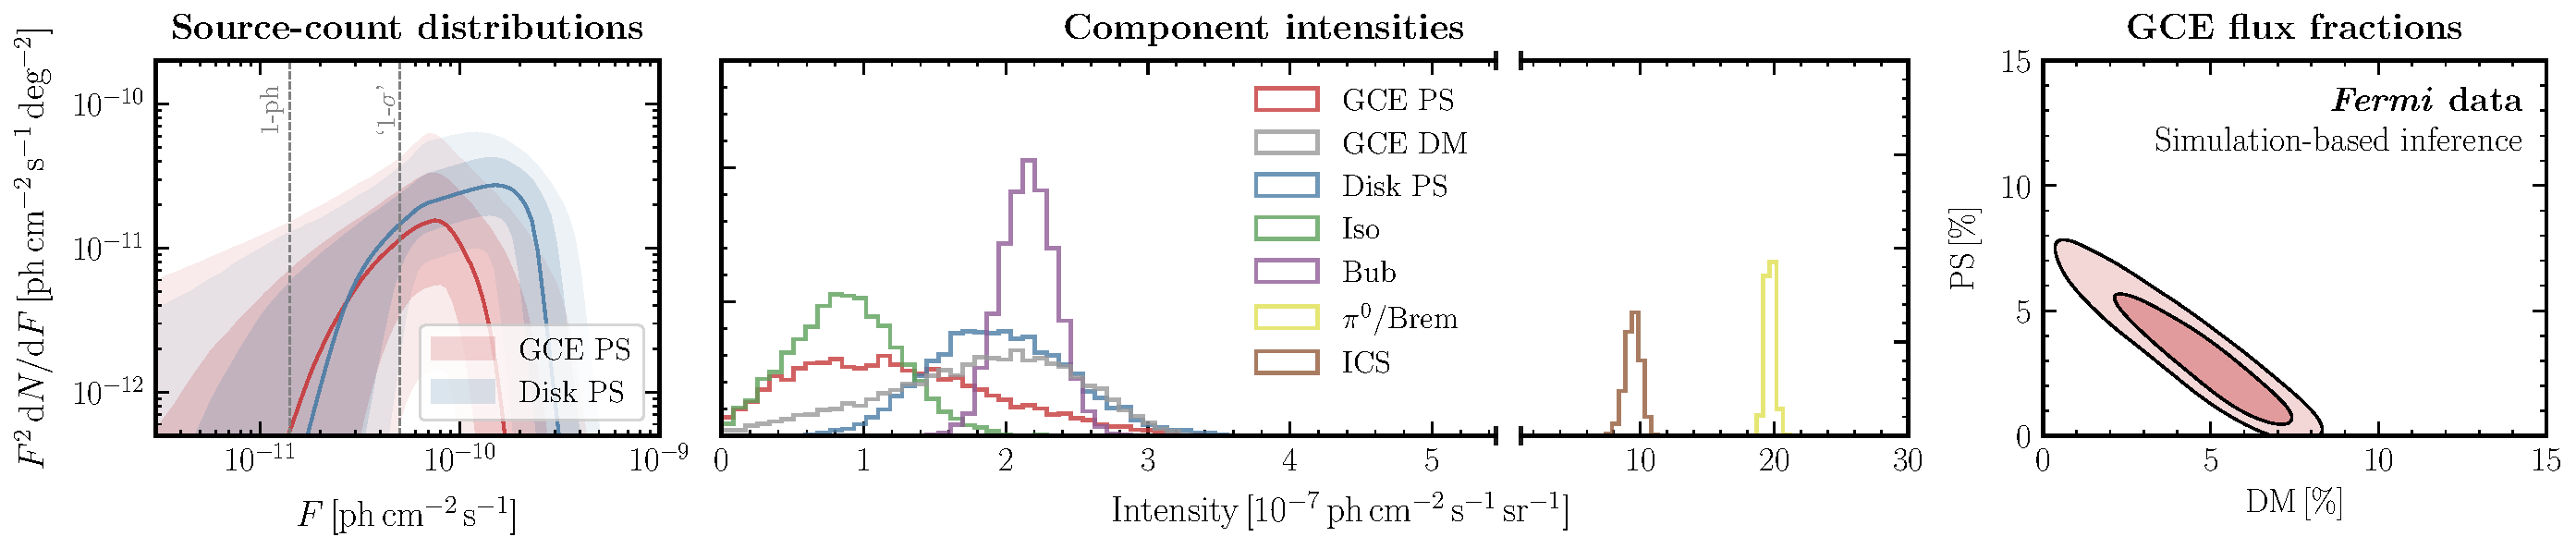
\includegraphics[width=0.95\textwidth]{figures/data_fid_sbi.pdf} \\
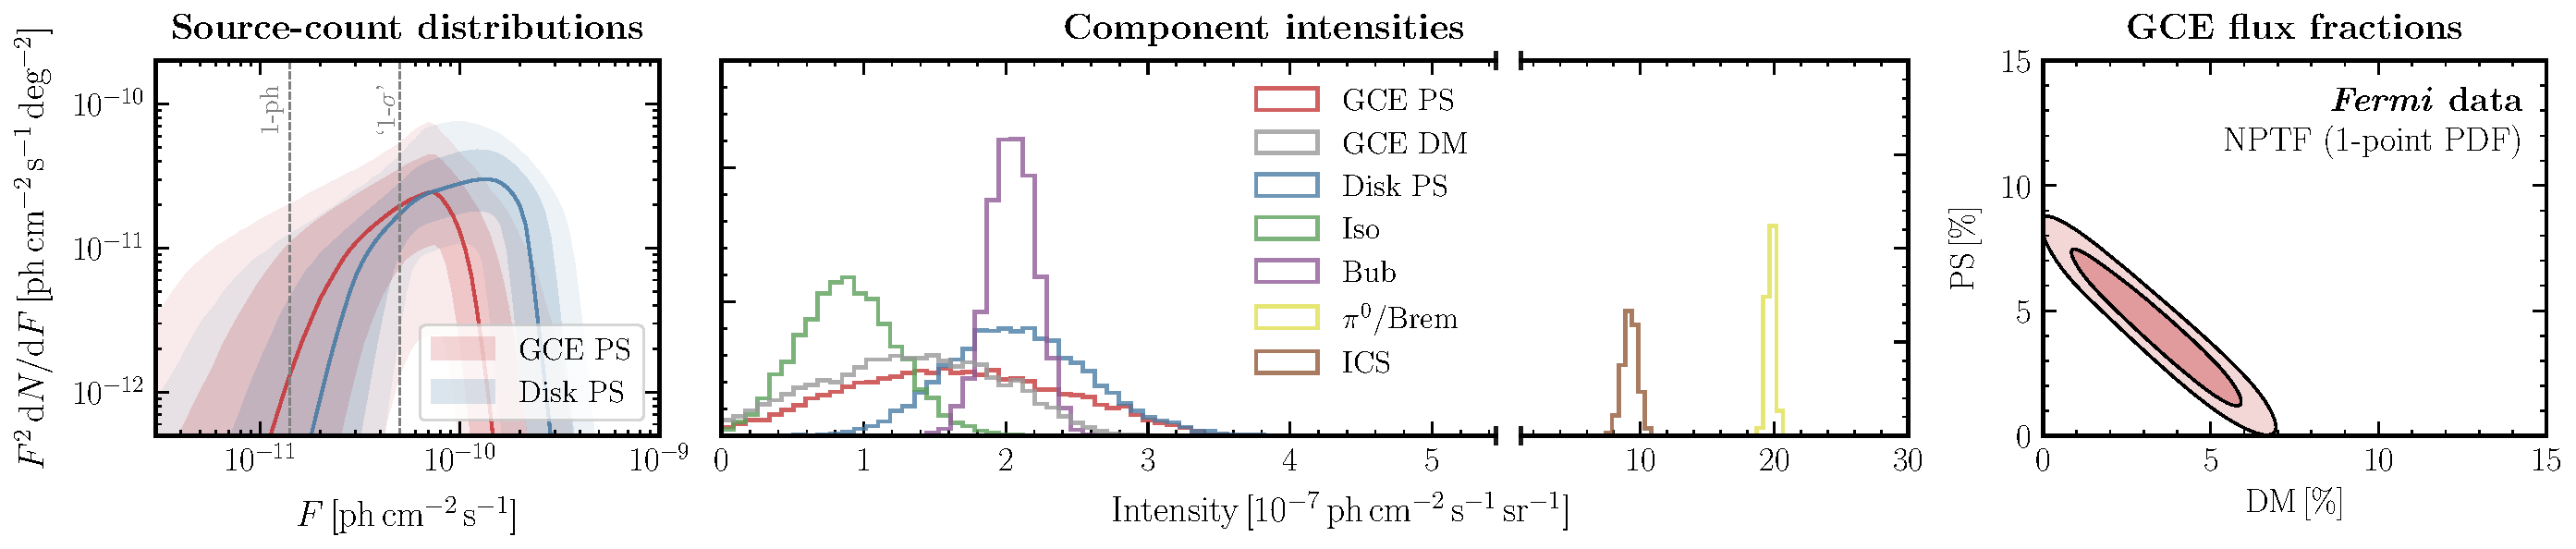
\includegraphics[width=0.95\textwidth]{figures/data_fid_nptf.pdf}
\caption{Results of the baseline analysis on real \Fermi data. \emph{(Top row)} Analysis using neural simulation-based inference with normalizing flows, and \emph{(bottom row)} using the 1-point PDF likelihood implemented in the non-Poissonian template fitting (NPTF) framework. While moderate preference for a PS-like origin of the GCE is seen in the case of the NPTF analysis (bottom), the simulation-based inference analysis attributes a smaller fraction of the GCE to PS-like emission (top).}
\label{fig:fid_data}
\end{figure}
%

We apply our neural simulation-based inference pipeline to the real \Fermi dataset. As a point of comparison, we also run the NPTF method on the data using the same spatial templates and prior assumptions as those used in the corresponding SBI analyses. 
The results of the NPTF analysis are shown in the bottom panel of Fig.~\ref{fig:fid_data}. The left column shows the median (solid lines) as well as middle-68/95\% containment (dark/light shaded regions) of the posteriors on the source-count distributions $F^2 \dd N/\dd F$ of GCE-correlated (red) and disk-correlated (blue) PSs, evaluated point-wise in flux $F$. The dashed grey vertical lines correspond to the flux associated with a single expected photon count per source (below which Poissonian and PS-like emission is expected to be perfectly degenerate) and the approximate 1-$\sigma$ threshold for detecting individual sources (below which the degeneracy is often observed in practice~\cite{Chang:2019ars,Buschmann:2020adf}). The middle column shows the posteriors on various modeled emission components.
% , excluding emission from resolved 3FGL PSs as the posterior in that case is largely unconstrained owing to the fact that resolved PSs are masked out in the analysis. 
The right column shows the joint posterior on the fraction of DM- and PS-like emission in proportion to the total inferred flux in the ROI.

Consistent with previous 1-point PDF studies using a similar configuration, a significant fraction of the GCE---$55.0^{+8.8}_{-22.9}\%$--is attributed to PS-like emission.
The top panel of Fig.~\ref{fig:fid_data} shows results using the neural simulation-based analysis pipeline introduced in this paper. Although posteriors for the astrophysical background templates are seen to be broadly consistent with those inferred in the NPTF analysis, the preference for PSs is somewhat reduced in this case, with $32.5^{+9.1}_{-18.7}\%$ of the GCE emission being PS-like. 

% We also note that, in both cases, the inferred GCE-correlated source-count distribution peaks at lower values than those inferred in previous NPTF analyses, which have generally found the bulk of expected emission from PSs to lie just below the 3FGL PS detection threshold~\cite{Lee:2015fea} at $\sim2$--$3\times 10^{-10}$\,ph\,cm$^{-2}$\,s$^{-1}$. In this baseline configuration, the SCD peak is constrained to be $2.3^{+1.2}_{-2.2}\times 10^{-11}$\,ph\,cm$^{-2}$\,s$^{-1}$. We note that that the position of the SCD peak is related to the flux at which the largest number of PSs are inferred to lie, rather than a statement about which fluxes the majority of the emission comes from.

\section{Discussion}
\label{sec:conclusions}

We have leveraged recent advances in neural simulation-based inference in order to jointly characterize a putative DM-like signal and PS population associated with the observed \Fermi Galactic Center Excess. While broadly consistent with results of the traditional method, our method shows a reduced preference for PS-like emission correlated with the GCE. In our extended work~\cite{Mishra-Sharma:InProgress}, we present additional details of our analysis, including a validation of our pipeline on simulated data as well as a discussion of the impact of model misspecification within our framework. We show there that, owing to the fact that it can extract more information from the forward model, our method is less sensitive to certain forms of model misspecification than traditional approaches.

As in any Galactic Center $\gamma$-ray analysis, we caution of the potential of unknown systematics, such as mismodeling on the scale of the size of the \Fermi point-spread function, to bias the results and conclusions of our analysis. Although machine learning-based analyses can utilize more of the information encoded in the forward model, and in particular in the present case can take advantage of pixel-to-pixel correlations, this can also make them more susceptible to specific modeled features compared to traditional techniques based on data reduction to hand-crafted data summaries. We leave a more detailed investigation of the impact of these effects to future work.

Code used for reproducing the results presented in this paper is available at \url{https://github.com/smsharma/fermi-gce-flows}. 

\begin{ack}
SM benefitted from the hospitality of the Center for Computational Astrophysics at the Flatiron Institute while this work was being performed. 
This work was performed in part at the Aspen Center for Physics, which is supported by National Science Foundation grant PHY-1607611.
The participation of SM at the Aspen Center for Physics was supported by the Simons Foundation.
SM is supported by the NSF CAREER grant PHY-1554858, NSF grants PHY-1620727 and PHY-1915409, and the Simons Foundation. 
This work is supported by the National Science Foundation under Cooperative Agreement PHY-2019786 (The NSF AI Institute for Artificial Intelligence and Fundamental Interactions, \url{http://iaifi.org/}).
This work made use of the NYU IT High Performance Computing resources, services, and staff expertise. 
This research has made use of NASA's Astrophysics Data System. 
This research made use of the Astropy~\cite{Robitaille:2013mpa,Price-Whelan:2018hus},
healpy~\cite{Gorski:2004by,Zonca2019},
IPython~\cite{PER-GRA:2007},
Jupyter~\cite{Kluyver2016JupyterN},
Matplotlib~\cite{Hunter:2007},
NumPy~\cite{harris_array_2020},
PyTorch~\cite{NEURIPS2019_9015},
SciPy~\cite{2020SciPy-NMeth}, and
Seaborn~\cite{michael_waskom_2017_883859}
software packages.
\end{ack}

\bibliographystyle{apsrev4-1-mod}

{
\small
\bibliography{fermi-gce-flows}
}

%%%%%%%%%%%%%%%%%%%%%%%%%%%%%%%%%%%%%%%%%%%%%%%%%%%%%%%%%%%%
\section*{Checklist}

\begin{enumerate}

\item For all authors...
\begin{enumerate}
  \item Do the main claims made in the abstract and introduction accurately reflect the paper's contributions and scope?
    \answerYes{}
  \item Did you describe the limitations of your work?
    \answerYes{See Sec.~\ref{sec:conclusions}}
  \item Did you discuss any potential negative societal impacts of your work?
    \answerNA{Potential negative societal impacts were considered, and we believe this work does not present any issues in this regard.}
  \item Have you read the ethics review guidelines and ensured that your paper conforms to them?
    \answerYes{}
\end{enumerate}

\item If you are including theoretical results...
\begin{enumerate}
  \item Did you state the full set of assumptions of all theoretical results?
    \answerNA{No theoretical results were obtained in this work.}
	\item Did you include complete proofs of all theoretical results?
    \answerNA{}
\end{enumerate}

\item If you ran experiments...
\begin{enumerate}
  \item Did you include the code, data, and instructions needed to reproduce the main experimental results (either in the supplemental material or as a URL)?
    \answerYes{The code repository associated with this paper and needed to reproduce all the results is linked in Sec.~\ref{sec:conclusions}.}
  \item Did you specify all the training details (e.g., data splits, hyperparameters, how they were chosen)?
    \answerYes{These are described in Sec.~\ref{sec:experiments}.}
	\item Did you report error bars (e.g., with respect to the random seed after running experiments multiple times)?
    \answerYes{}
	\item Did you include the total amount of compute and the type of resources used (e.g., type of GPUs, internal cluster, or cloud provider)?
    \answerNo{Due to space constraints limiting the total length of the extended abstract to 4 pages, this information will be included in the camera-ready version of the paper.}
\end{enumerate}

\item If you are using existing assets (e.g., code, data, models) or curating/releasing new assets...
\begin{enumerate}
  \item If your work uses existing assets, did you cite the creators?
    \answerYes{All code used for this project is cited in the Acknowledgments section, which is redacted during blind review. Code citations will be reinstated for the camera-ready version of the paper.} 
  \item Did you mention the license of the assets?
    \answerNA{Licenses are mentioned in the links associated with individual code packages.}
  \item Did you include any new assets either in the supplemental material or as a URL?
    \answerNA{No new assets (excluding the code used to reproduced the experiments) were produced in this work.}
  \item Did you discuss whether and how consent was obtained from people whose data you're using/curating?
    \answerNA{}
  \item Did you discuss whether the data you are using/curating contains personally identifiable information or offensive content?
    \answerNA{No personal information is included in the assets utilized in this paper.}
\end{enumerate}

\item If you used crowdsourcing or conducted research with human subjects...
\begin{enumerate}
  \item Did you include the full text of instructions given to participants and screenshots, if applicable?
    \answerNA{}
  \item Did you describe any potential participant risks, with links to Institutional Review Board (IRB) approvals, if applicable?
    \answerNA{}
  \item Did you include the estimated hourly wage paid to participants and the total amount spent on participant compensation?
    \answerNA{}
\end{enumerate}

\end{enumerate}

%%%%%%%%%%%%%%%%%%%%%%%%%%%%%%%%%%%%%%%%%%%%%%%%%%%%%%%%%%%%

\end{document}